\begin{frame}{Monte Carlo Tree Search(MCTS)}{Quesque le MCTS}
	\begin{block}{}
		\begin{itemize}
			\item Le MCTS est un algorithme de recherche arborescente utilisé pour résoudre des problèmes afin de prendre une décision (un déplacement dans un jeu par exemple).
			\item Il n'utilise pas de fonction d'évaluation heuristique comparé à $\alpha$$\beta$ par exemple, et parcours les possibilités aléatoirement, en utilisant les donnés obtenus précédemment			\item Il utilise les méthodes de Monte Carlo pour améliorer son efficacité.
			\item Il possède des variantes, dépendant de leur utilisation, comme Coulom ou Kocsis and Szepesvari par exemple.
			\item Applicable si toutes les règles de l'application sont connus et si la longueur d'une partie et les gains ont une limite.	
		\end{itemize}
	\end{block}
\end{frame}

\begin{frame}{Monte Carlo Tree Search(MCTS)}{Structure}
	\begin{block}{Arbre de recherche}
		\begin{itemize}
			\item L'arbre de recherche est une modélisation des possibilités de jeu pour la simulation.
			\item Un noeud représente un état du jeu.
			\item Chaque noeuds possèdent deux informations :
			\item\begin{itemize}
				\item - La valeur de sa position (dans un jeu, représenté souvent par la moyenne des résultats pour un jeu sur les noeuds visités).
				\item - Le nombre de visite de ce noeud dans la simulation.
			\end{itemize}
			\item Chaque feuille de cet arbre représente soit un noeud dont les enfants n'ont pas encore été explorés, soit un état final de celui-ci.		
		\end{itemize}
	\end{block}
\end{frame}

\begin{frame}{Monte Carlo Tree Search(MCTS)}{Structure}
    \begin{block}{Plusieurs étapes}
	    	\begin{itemize}
	    		\item 1. Sélection
	    		\item 2. Expansion
	    		\item 3. Simulation
	    		\item 4. Rétropropagation
	    		\item Répété jusqu'à un certain temps jusqu'à la prise de décision.
	    	\end{itemize}
		\begin{center}
			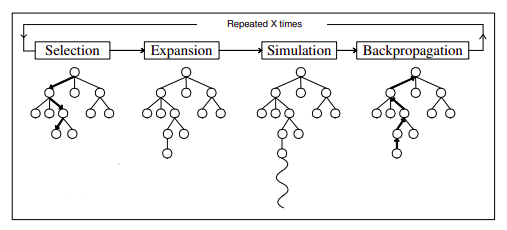
\includegraphics[width=8cm]{ressources/MCTSEtapes}
		\end{center}
	\end{block}
\end{frame}

\begin{frame}{Monte Carlo Tree Search(MCTS)}{Sélection}
\begin{block}{Fonctionnement}
	\begin{columns}
		\begin{column}{6cm}
			\begin{itemize}
				\item En commençant à partir de la racine, on applique récursivement une stratégie de sélection pour trouver une feuille de l'arbre à étendre (un chemin qui n'a donc pas encore été exploré).
				\item La stratégie doit pour optimiser les résultats, faire un consensus entre exploitation et exploration.
				\item Il existe pour cela plusieurs stratégies comme OMC, UCT, PBBM, ...
			\end{itemize}
		\end{column}
		\begin{column}{3cm}
			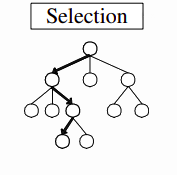
\includegraphics[width=3cm]{ressources/Selection.png}
		\end{column}
	\end{columns}
\end{block}
\end{frame}

\begin{frame}{Monte Carlo Tree Search(MCTS)}{Stratégie Sélection}
	\begin{block}{Stratégie OMC (Objective Monte-Carlo)}
		\begin{itemize}
			\item $U_{i}$ une fonction d'urgence d'un mouvement avec :
			\item $U_{i} = erfc(\frac{v_{0} - v_{i}}{\sqrt{2}\sigma_{i}})$
			\item $v_{0}$ la valeur du meilleur mouvement et $v_{j}$ la valeur du mouvement courant.
			\item $\sigma_{j}$ la déviation de $v_{j}$
			\item erfc la fonction complémentaire d'erreur avec :
			\item $erfc(x) = 1 - \frac{2}{\sqrt{\pi}}\int_{x}^{\infty}e^{-u^{2}}$
			\item La probabilité $P_{m}$ pour chaque $m \in M$ avec :
			\item $P_{m} = \frac{U(m)}{\sum_{j \in S_{i}}^{}U(j)}$
			\item On choisit le prochain mouvement à simuler aléatoirement selon la probabilité $P_{m}$ et peut être longue à calculer.
		\end{itemize}
	\end{block}
\end{frame}

\begin{frame}{Monte Carlo Tree Search(MCTS)}{Stratégie Sélection}
	\begin{block}{PBBM (Probability to be Better than Best Move)}
		\begin{itemize}
			\item Similitude avec la stratégie OMC
			\item $U_{i}$ aussi une fonction d'urgence d'un mouvement avec :
			\item $U_{i} = \exp(-2.4\frac{v_{0} - v_{i}}{\sqrt{2(\sigma_{0}^2 + \sigma_{i}^2)}})) + \epsilon_{i}$
			\item $v_{0}$ la valeur du meilleur mouvement et $v_{i}$ la valeur du mouvement courant.
			\item $\sigma_{0}$ et $\sigma_{i}$ leur déviations
			\item $\epsilon_ {i}$ une constante assurant que la fonction d'urgence ne soit pas égale à 0 avec :
			\item $\epsilon_ {i} = \frac{0.1 + 2^{-i} + a_{i}}{N}$
			\item $a_{i} = 1$ si le mouvement est un atari et $0$ sinon 
		\end{itemize}
	\end{block}
\end{frame}

\begin{frame}{Monte Carlo Tree Search(MCTS)}{Stratégie Sélection}
	\begin{block}{Stratégie UCT (Upper Confidence bounds applied to Trees)}
		\begin{itemize}
			\item La stratégie UCT sélectionne un noeud $k$ fils du noeud $p$ qui satisfait la formule suivante :
			\item $k \in argmax_{i\in I}(v_{i} + C \times \sqrt{\frac{\ln n_{p}}{n_{i}}})$
			\item $I$ un set de noeuds atteignable par le noeud $p$.
			\item $v_{i}$ la valeur du noeud i
			\item $n_{p}$ et $n_{p}$ le nombre de fois que les noeuds $p$ et $i$ on été visités.
			\item $C$ une constante.
			\item Facile à implémenter et beaucoup utilisée.
		\end{itemize}
	\end{block}
\end{frame}

\begin{frame}{Monte Carlo Tree Search(MCTS)}{Stratégie Sélection}
	\begin{block}{Stratégie UCB1-TUNED}
		\begin{itemize}
			\item Variante de la stratégie UCT
			\item Cette sélectionne un noeud $k$ fils du noeud $p$ qui satisfait la formule suivante :
			\item $k \in argmax_{i\in I}(v_{i} + C \times \sqrt{\frac{\ln n_{p}}{n_{i}}\times \min(\frac{1}{4}, V_{i}(n_{i}))})$
			\item avec $V_{i}$ une estimation de la borne supérieur de la variance de $v_{i}$ avec comme formule :
			\item $V_{i}(n_{i}) = (\frac{1}{n_{i}}\sum_{t=1}^{n_{i}}R_{i,t,j}^2 - v_{i}^2 + \sqrt{\frac{2\ln n_{p}}{n_{i}}})$
			\item $R_{i,t,k}$ la t-ième récompense obtenu au noeud $i$ pour le joueur $j$
		\end{itemize}
	\end{block}
\end{frame}

\begin{frame}{Monte Carlo Tree Search(MCTS)}{Expansion}
	\begin{block}{Fonctionnement}
		\begin{columns}
			\begin{column}{8cm}
				\begin{itemize}
					\item Dépendant des règles du jeu, crée un noeud à partir du noeud sélectionné si celui-ci n'est pas final.
					\item On ne peut pas garder tout les résultats en mémoire.
					\item Il existe plusieurs stratégies pour garder en mémoire les noeuds comme par exemple garder seulement un noeud par jeu simulé. Ce noeud correspond à la première position qui n'étaient pas déjà stockées lors du parcours.
				\end{itemize}
			\end{column}
			\begin{column}{4cm}
				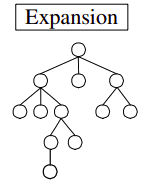
\includegraphics[width=3cm]{ressources/Expansion.png}
			\end{column}
		\end{columns}
	\end{block}
\end{frame}

\begin{frame}{Monte Carlo Tree Search(MCTS)}{Simulation}
	\begin{block}{Fonctionnement}
		\begin{columns}
			\begin{column}{7cm}
				\begin{itemize}
					\item Cette étape réalise une simulation d'une partie aléatoirement (ou partiellement) à partir du noeud qui à été étendu jusqu'à atteindre un état final, afin d'obtenir un résultat.
					\item Il existe des stratégies de simulation, mais qui sont difficile à définir car on doit garder un bon compromis entre recherche et exploitation.
					\item Ces stratégies peuvent utilises des connaissances du jeu (patterns, considérations, ...)
				\end{itemize}
			\end{column}
			\begin{column}{4cm}
				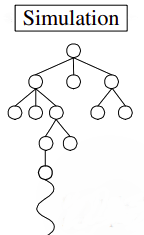
\includegraphics[width=3cm]{ressources/Simulation.png}
			\end{column}
		\end{columns}
	\end{block}
\end{frame}

\begin{frame}{Monte Carlo Tree Search(MCTS)}{Stratégie Simulation}
	\begin{block}{Exemple d'une stratégie : Sequence-like Simulation}
		\begin{itemize}
			\item Cette stratégie est adapté au jeu de GO.
			\item Dans cette statégie, on sélectionne chaque coup à proximité du dernier coup joué, afin de créer une séquence de coups adjacent. On sélectionne le coup à jouer dans la séquence du dernier coup en cherchant des motifs de jeu de taille 3x3 à une distance 1 par rapport au dernier coup. Ces motifs doivent être réalisés avec des connaissances du jeu. Si plusieurs motifs correspondent, on choisis aléatoirement le motif en jouant au milieu de celui-ci. Si aucun est reconnu, on choisit aléatoirement le coup.
			\item (Distance de Manhattan : $d(A,B) = |X_{B} - X_{A}| + |Y_{B} - Y_{A}|$ dit aussi la distance entre deux points parcourue par un taxi lorsqu'il se déplace dans une ville où les rues sont agencées selon un réseau ou quadrillage.)
		\end{itemize}
	\end{block}
\end{frame}

\begin{frame}{Monte Carlo Tree Search(MCTS)}{Rétropropagation}
	\begin{block}{Fonctionnement}
		\begin{columns}
			\begin{column}{8cm}
				\begin{itemize}
					\item La rétropropagation utilise le résultat de la simulation pour propager l'information aux parents de ce noeud récursivement jusqu'au plus haut afin de les mettre à jour, changeant alors la valeur des noeud. 
					\item Le résultat pour un jeu à deux joueurs comme le GO peut être interprété de la façon suivante avec $R_{i}$ ce résultat : Si le joueur que joue l'IA gagne, $R_{i} = +1$, si il perd, $R_{i} = -1$ et $0$ sinon.
					\item Il existe aussi plusieurs stratégie de rétropropagation.
				\end{itemize}
			\end{column}
			\begin{column}{4cm}
				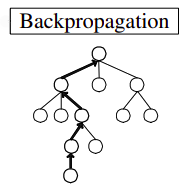
\includegraphics[width=3cm]{ressources/Backpropagation.png}
			\end{column}
		\end{columns}
	\end{block}
\end{frame}

\begin{frame}{Monte Carlo Tree Search(MCTS)}{Stratégie Rétropropagation}
	\begin{block}{Exemple de stratégies}
		\begin{itemize}
			\item \textbf{Moyenne} : Prend la moyenne des résultats : $v_{i} = \frac{\sum_{i}^{}R_{i}}{n_{i}}$ avec $v_{i}$ la valeur du noeud et $n_i$ le nombre de fois qu'il a été visité.
			\item \textbf{Max} : Prend le max des résultats des enfants (pas efficace)
			\item \textbf{Moyenne informée} : Attribue de plus grande valeur aux meilleurs résultats afin d'avoir le meilleurs résultats plus rapidement.
			On a : $v_{i} = \frac{\sum_{j}^{}(v_{j}\times n_{j}\times U_{j})}{\sum_{j}^{}(n_{j}\times U_{j})}$ avec $U_{j}$ la fonction d'urgence utilisé pour la stratégie de séléction OMC.
			\item Mais la majorité des programmes utilise la stratégie \textbf{Average} car elle donne de meilleurs résultats.
		\end{itemize}
	\end{block}
\end{frame}

\begin{frame}{Monte Carlo Tree Search(MCTS)}{Choix du mouvement final}
	\begin{block}{Exemple de choix du mouvement}
		\begin{itemize}
			\item \textbf{Maximum des noeuds}: On prend le noeud qui a la plus grande valeur.
			\item \textbf{Noeud le plus robuste}: On prend le noeud qui a été visité le plus de fois.
			\item \textbf{Mix}: On prend le noeud qui est à la fois le maximum et le plus robuste (on fait des simulations jusqu'à en obtenir un si non existant)
			\item \textbf{Noeud le plus sécurisé}: On prend le noeud qui maximise une borne de confiance (a besoin d'expérimentation).
			\item Il n'y pas beaucoup de différence parmi ces choix, sauf lorsque le temps pour faire le choix est faible, où le choix max devient moins efficace.
		\end{itemize}
	\end{block}
\end{frame}

\begin{frame}{Monte Carlo Tree Search(MCTS)}{Application}
	\begin{block}{Exemple d'applications}
		\begin{itemize}
			\item Pour les jeux à deux joueurs comme pour le GO, le MCTS a été une révolution :
			\item Le programme MCTS Mogo Titan a permis pour la première fois de battre un joeurs pro de Go avec contrainte (7 pierres d'handicap).
			\item Utilisés par les programmes MOGO, CRAZY STONE, FUEGO, ... qui sont aussi très efficace.
			\item AlphaGo utilise aussi le MCTS pour sa recherche de coup (en l'adaptant à son programme).
			
		\end{itemize}
	\end{block}
\end{frame}